%Notes by Harsh Mistry 
%Math 239
%based on Template from : https://www.cs.cmu.edu/~ggordon/10725-F12/template.tex

\documentclass{article}
\setlength{\oddsidemargin}{0.25 in}
\setlength{\evensidemargin}{-0.25 in}
\setlength{\topmargin}{-0.6 in}
\setlength{\textwidth}{6.5 in}
\setlength{\textheight}{8.5 in}
\setlength{\headsep}{0.75 in}
\setlength{\parindent}{0 in}
\setlength{\parskip}{0.1 in}
\usepackage{amsfonts,graphicx, amssymb}
\usepackage[fleqn]{amsmath}
\usepackage{fixltx2e}
\usepackage{color}
\usepackage{tcolorbox}
\usepackage{lipsum}
\usepackage{listings}
\usepackage{scrextend}
\tcbuselibrary{skins,breakable}
\usetikzlibrary{shadings,shadows}
\usepackage{graphicx}
\graphicspath{ {images/} }
\newcounter{lecnum}
\renewcommand{\thepage}{\thelecnum-\arabic{page}}
\renewcommand{\thesection}{\thelecnum.\arabic{section}}
\renewcommand{\theequation}{\thelecnum.\arabic{equation}}
\renewcommand{\thefigure}{\thelecnum.\arabic{figure}}
\renewcommand{\thetable}{\thelecnum.\arabic{table}}
\newcommand{\lecture}[4]{
   \pagestyle{myheadings}
   \thispagestyle{plain}
   \newpage
   \setcounter{lecnum}{#1}
   \setcounter{page}{1}
   
   
%Info Box 
   \begin{center}
   \framebox{
      \vbox{\vspace{2mm}
    \hbox to 6.28in { {\bf Math 239 - Introduction to Combinatorics
	\hfill Spring 2017} }
       \vspace{4mm}
       \hbox to 6.28in { {\Large \hfill Lecture #1: #2  \hfill} }
       \vspace{2mm}
       \hbox to 6.28in { {\it Lecturer: #3 \hfill Notes By: #4} }
      \vspace{2mm}}
   }
   \end{center}
   
   \markboth{Lecture #1: #2}{Lecture #1: #2}



 
}

\renewcommand{\cite}[1]{[#1]}
\def\beginrefs{\begin{list}%
        {[\arabic{equation}]}{\usecounter{equation}
         \setlength{\leftmargin}{2.0truecm}\setlength{\labelsep}{0.4truecm}%
         \setlength{\labelwidth}{1.6truecm}}}
\def\endrefs{\end{list}}
\def\bibentry#1{\item[\hbox{[#1]}]}

\newcommand{\fig}[3]{
			\vspace{#2}
			\begin{center}
			Figure \thelecnum.#1:~#3
			\end{center}
	}
	
	\newcommand{\bs}{
		\texttt{\char`\\ \hspace{0.1cm}} 
	}
	

	
\newcommand{\pipe}{\(\mid\)}
\newcommand{\ctr}{\(\wedge\)}

\newtheorem{theorem}{Theorem}[lecnum]
\newtheorem{lemma}[theorem]{Lemma}
\newtheorem{ex}[theorem]{Example}
\newtheorem{expx}[theorem]{Problem}
\newtheorem{prop}[theorem]{Proposition}
\newtheorem{claim}[theorem]{Claim}
\newtheorem{corollary}[theorem]{Corollary}
\newtheorem{definition}[theorem]{Definition}
\newenvironment{proof}{{\bf Proof:}}{\hfill\rule{2mm}{2mm}}
\newcommand\E{\mathbb{E}}

%color definitions :
\definecolor{darkred}{rgb}{0.55, 0.0, 0.0}
\definecolor{lightcoral}{rgb}{0.94, 0.5, 0.5}
\definecolor{tomato}{rgb}{1.0, 0.39, 0.28}
\definecolor{lightgray}{rgb}{.9,.9,.9}
\definecolor{darkgray}{rgb}{.4,.4,.4}
\definecolor{purple}{rgb}{0.65, 0.12, 0.82}
\definecolor{lightgreen}{rgb}{0.56, 0.93, 0.56}
\definecolor{darkgreen}{rgb}{0.0, 0.2, 0.13}
\definecolor{limegreen}{rgb}{0.2, 0.8, 0.2}
\definecolor{lightblue}{rgb}{0.68, 0.85, 0.9}
\definecolor{darkblue}{rgb}{0.0, 0.0, 0.55}


%Environments
\newenvironment{exblock}[1]{%
    \tcolorbox[beamer,%
    noparskip,breakable,
    colback=lightgreen,colframe=darkgreen,%
    colbacklower=limegreen!75!lightgreen,%
    title=#1]}%
    {\endtcolorbox}

\newenvironment{ablock}[1]{%
    \tcolorbox[beamer,%
    noparskip,breakable,
    colback=lightcoral,colframe=darkred,%
    colbacklower=tomato!75!lightcoral,%
    title=#1]}%
    {\endtcolorbox}

\newenvironment{cblock}[1]{%
    \tcolorbox[beamer,%
    noparskip,breakable,
    colback=lightblue,colframe=darkblue,%
    colbacklower=darkblue!75!lightblue,%
    title=#1]}%
    {\endtcolorbox}


%Languages
\lstdefinelanguage{JavaScript}{
  keywords={typeof, new, true, false, catch, function, return, null, catch, switch, var, if, in, while, do, else, case, break},
  keywordstyle=\color{blue}\bfseries,
  ndkeywords={class, export, boolean, throw, implements, import, this},
  ndkeywordstyle=\color{darkgray}\bfseries,
  identifierstyle=\color{black},
  sensitive=false,
  comment=[l]{//},
  morecomment=[s]{/*}{*/},
  commentstyle=\color{purple}\ttfamily,
  stringstyle=\color{red}\ttfamily,
  morestring=[b]',
  morestring=[b]"
}

%Listings
\lstset{
   language=JavaScript,
   backgroundcolor=\color{lightgray},
   extendedchars=true,
   basicstyle=\footnotesize\ttfamily,
   showstringspaces=false,
   showspaces=false,
   numbers=left,
   numberstyle=\footnotesize,
   numbersep=9pt,
   tabsize=2,
   breaklines=true,
   showtabs=false,
   captionpos=b
}


%Start
\begin{document}

\lecture{22}{June 19th, 2017}{Alan Arroyo Guevara}{Harsh Mistry}

\section{Eulerian Circuits}

\textbf{Eulers Question:} What graphs have a closed walk that contains all the edges of G exactly once?

Such walks are known as \textbf{Eulerian tours}

\begin{theorem}
(Euler) A connected graph has an Euler Tour \(\iff\) every vertex has an even degree. 
\end{theorem}

\begin{proof}
In course notes
\end{proof}

\begin{ex} -\\
\begin{center}
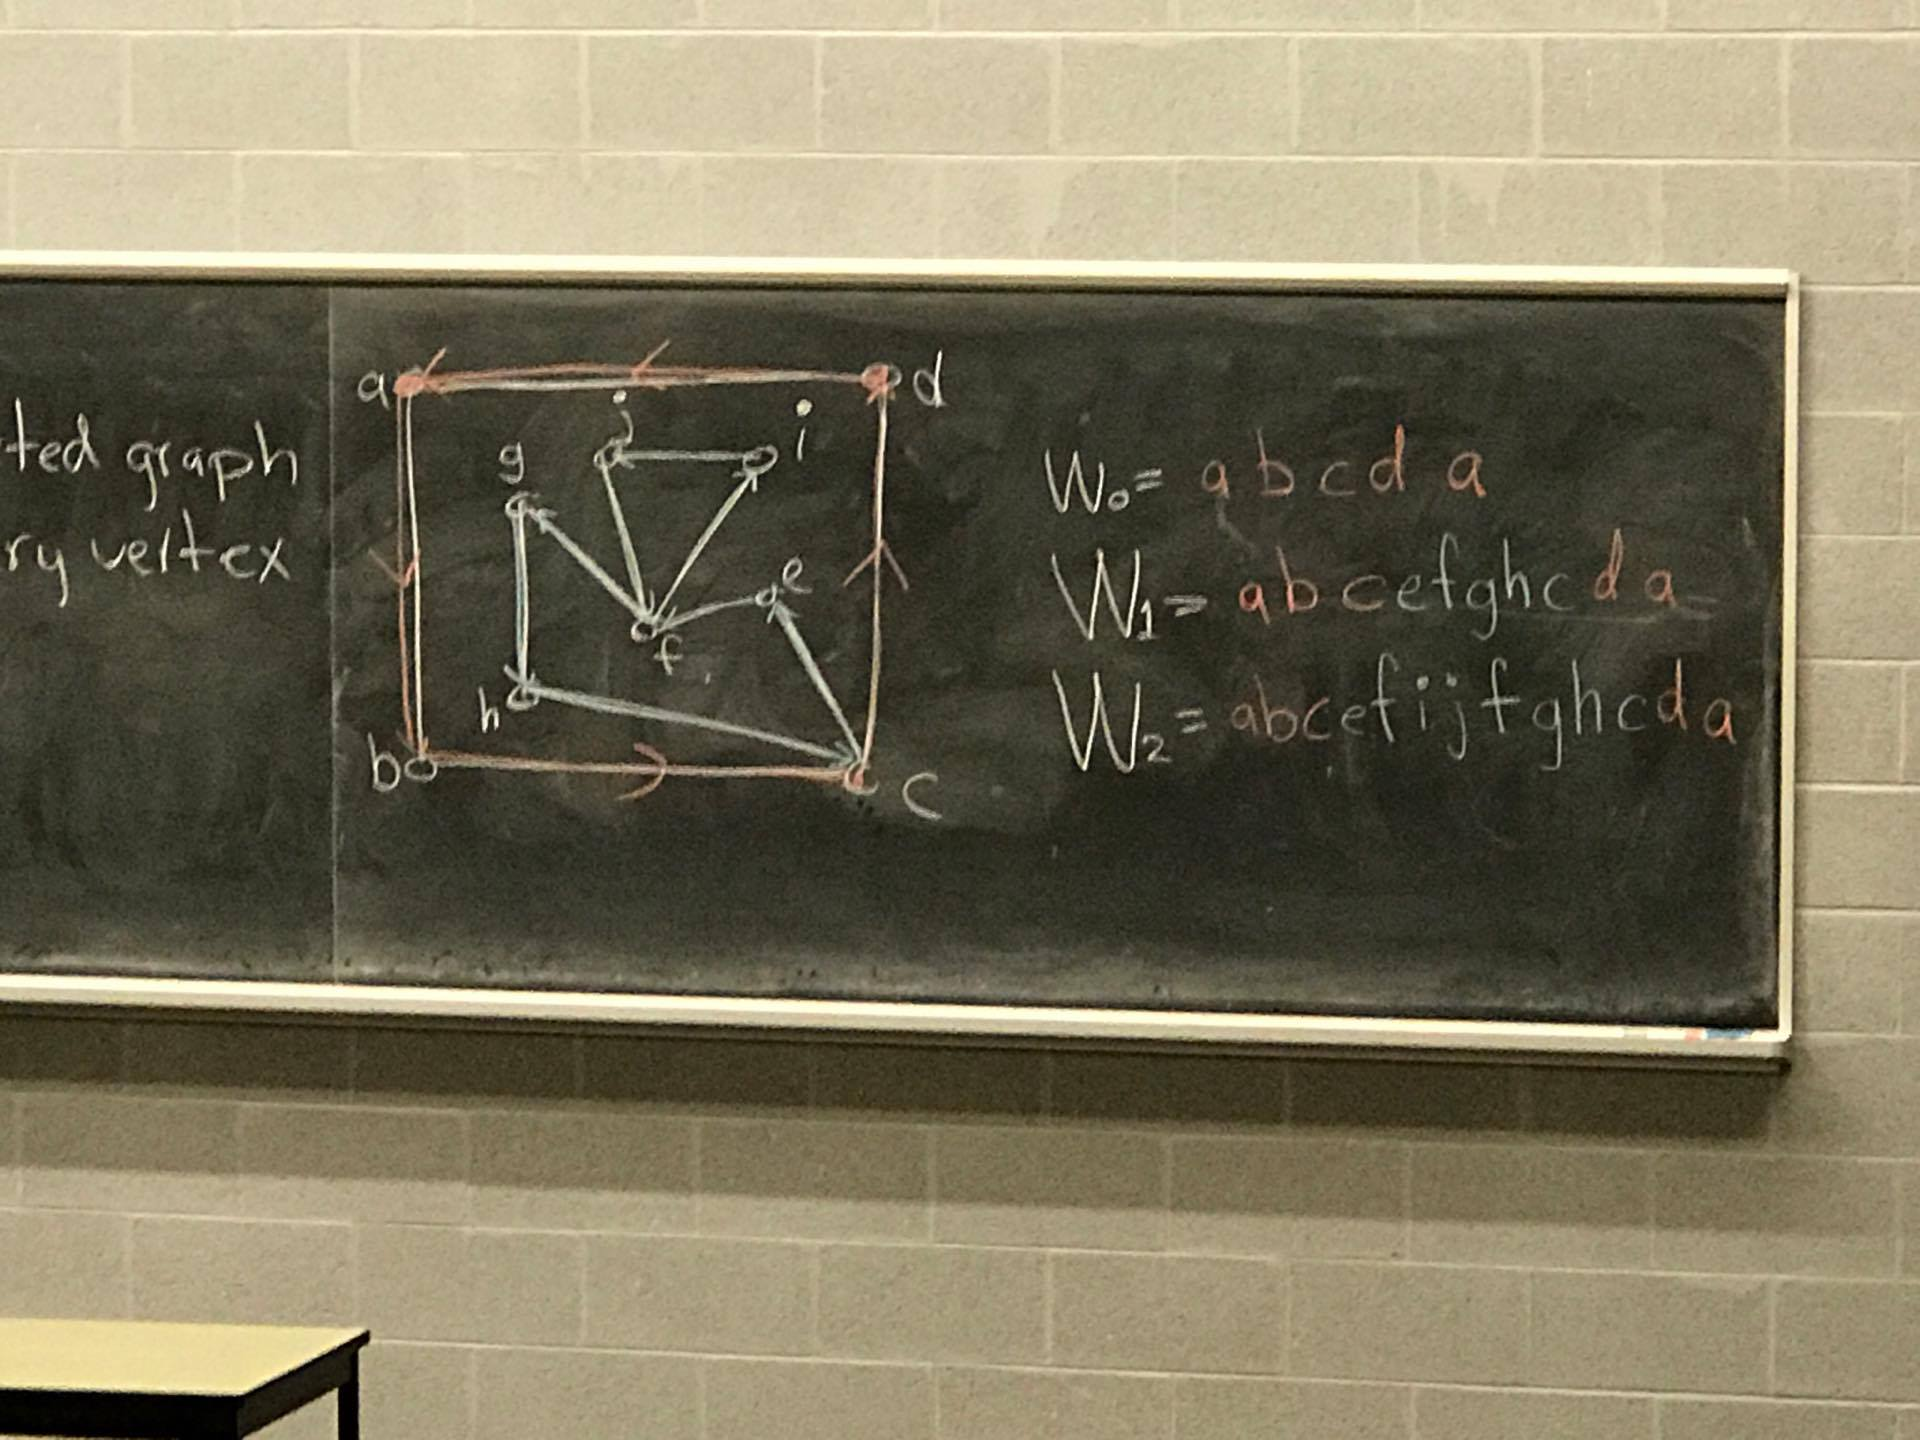
\includegraphics[scale=0.1]{13}
\end{center}
\end{ex}

\section{Trees}
\begin{definition}
A \textbf{tree} is a connected graph with no cycles
\end{definition}

\begin{lemma}
There is a unique path between vertices u and v in a tree T. 
\end{lemma}

\begin{proof}
Suppose there are two paths, \(P: x_0 x_1 \ldots x_n\) and \(Q : y_0 y_1 \ldots y_m\) where \(u = x_0 = y_0\) and \(v = x_n = y_m\)\\
\newline
Let \(i+1\) be the smallest index for which \(x_{i+1} \neq y_{i+1}\).\\ There is a closed walk connecting the ends of \(e: = x_i x_{i+1} \)that does not go through \(e: W\) is defined by following Q from \(y_i\) to \(y_m\) and then returning back from \(x_m\) to \(x_{i+1}\). \\
\newline
Since \(x_i\) and \(x_{i+1}\) are connected in \(T - e\), then e is not a bridge \(implies\) there is a cycles in T containing e, thus contradicting that T is a tree
\end{proof}

\textbf{Observation :} Every edge of a tree is a bridge

\begin{theorem}
A tree T with \(\mid V(G) \mid \geq 2\) has atleast two vertices of degree 1
\end{theorem}


\begin{theorem}
If T is a tree \(\implies \mid E(T) \mid = \mid V(T) \mid  - 1\)
\end{theorem}

\begin{proof}
\begin{itemize}
\item [\textbf{Base :}] n= 1 and and n=2 holds
\item [\textbf{I.H :}] Suppose that every tree with \(n-1\) vertices has \(n-2\) edges. 
\item[\textbf{I.S :}] Let T be a tree with n vertices. By the previous theorem, T has vertex c such that \(deg(v) = 1\)

Next Lecture 
\end{itemize}
\end{proof}

\end{document} 